%%%%%%%%%%%%%%%%%%%%%%%%%%%%%%%%%%%%%%%%%%%%%%%%%%%%%%%%%%%%%%%%%%%%%%%%
\clearpage
\section{Plugin functions for multiple scattering models}
\label{ch:pluginsMSANS}

According to \cite{Schelten1980,Jensen2018} the multiple  small angle scattering signal can be computed from the single scattering approximation via the intermediate function $i_1(r)$.
\begin{align}\label{eq:MSAS_SchmatzSchelten}
 i_1(r) &= 2\pi t \int_0^\infty J_0(qr) \frac{\mathrm{d}\sigma_1}{\mathrm{d}\Omega}(q) q \mathrm{d}q =2\pi t \mathcal{H}_0\left[\frac{\mathrm{d}\sigma_1}{\mathrm{d}\Omega}(q)\right](\delta)= 4\pi^2 t \tilde{G}(r)\\
 i_m(r) &= e^{-i_1(0)/k_0^2}k_0^2\left(\exp\left(i_1(r)/k_0^2\right)-1\right) \\
        &= k_0^2\left[\exp\left(\frac{t}{k_0^2}\left(\tilde{G}(r)-\tilde{G}(0)\right)\right)-\exp\left(-\frac{t}{k_0^2}\tilde{G}(0)\right)\right]\\
 \frac{\mathrm{d}\sigma_m}{\mathrm{d}\Omega}(q)&= \frac{1}{2\pi t} \int_0^\infty J_0(qr) i_m(r) r \mathrm{d}r = \frac{1}{2\pi t} \mathcal{H}_0\left[i_m(r)\right](Q) \\
 k_0 &= \frac{2\pi}{\lambda}
\end{align}
where $\frac{\mathrm{d}\sigma_m}{\mathrm{d}\Omega}(q)$ is the measured scattering cross-section including multiple scattering contributions normalized on the sample volume and  corrected for absorption and incoherent scattering, i.e. corrected for all beam attenuation effects except coherent small angle scattering. $\frac{\mathrm{d}\sigma_1}{\mathrm{d}\Omega}(q)$ is the corresponding single scattering cross-section per volume.
It can be seen, that the intermediate function $i_1(r)$ is except a pre-factor identical to the projected correlation function $\tilde{G}(r)$ used in the theory of  SESANS or SEMSANS analysis from section \ref{ch:pluginsSESANS}
\begin{align}
i_1(r)&=\tilde{G}(r)\left(2\pi\right)^2t
\end{align}
At the moment all the analytical models for projected correlation functions SESANS from chapter \ref{ch:pluginsSESANS} are also now available as scattering curves including multiple scattering effects. To include multiple scattering effects the scale parameter will be for all models the total scattering cross-section per sample volume $\Sigma_t=\tilde{G}(0)(2\pi)^2=i_1(0)/t$. Furthermore all the models contain two parameters  depending on the experimental conditions, which are the used wavelength $\lambda$ and the sample thickness $t$. Similar to the arguments for SESANS \cite{Kohlbrecher2017} the units should be chosen so that  $\lambda$ has the reciprocal units of the scattering vector $q$, i.e.\ nm or {\AA}, and the thickness should have the reciprocal units the scattering-cross section per volume, which are normally supplied in units of cm$^{-1}$. By this parametrisation the intermediate function $i_m(r)$ reads as
\begin{align}
 i_m(r) &= k_0^2\left[\exp\left(t\lambda^2\Sigma_t\left(\frac{\tilde{G}(r)-\tilde{G}(0)}{\tilde{G}(0)}\right)\right)-\exp\left(-t\lambda^2\Sigma_t\right)\right]
 \label{eq:MSAS_via_Gz}
\end{align}

\newpage
\subsection{Multiple scattering of Spheres}

This function uses the analytical expression for projected correlation function $\tilde{G}_\mathrm{sph}(\delta)$ of monodisperse spheres as given in eq.\ \ref{eq:Gz_sph} together with eq.\ \ref{eq:MSAS_via_Gz} to calculate the scattering intensity considering multiple scattering effects.

\hspace{1pt}\\
\uline{Input Parameters for model \texttt{MSAS Spheres}:}\\
\begin{description}
\item[\texttt{R}] radius of sphere $R$
\item[\texttt{dummy}] not used
\item[\texttt{dummy}] not used
\item[\texttt{Sigma\_t}] total scattering $\Sigma_t$
\item[\texttt{t}] sample thickness $t$
\item[\texttt{lambda}] wavelength of the beam $\lambda$
\end{description}

\hspace{1pt}\\
\uline{Note:}
\begin{itemize}
\item the function \texttt{MSAS Spheres} should not be combined with a size distribution nor a structure factor.
\end{itemize}

\begin{figure}[htb]
\begin{center}
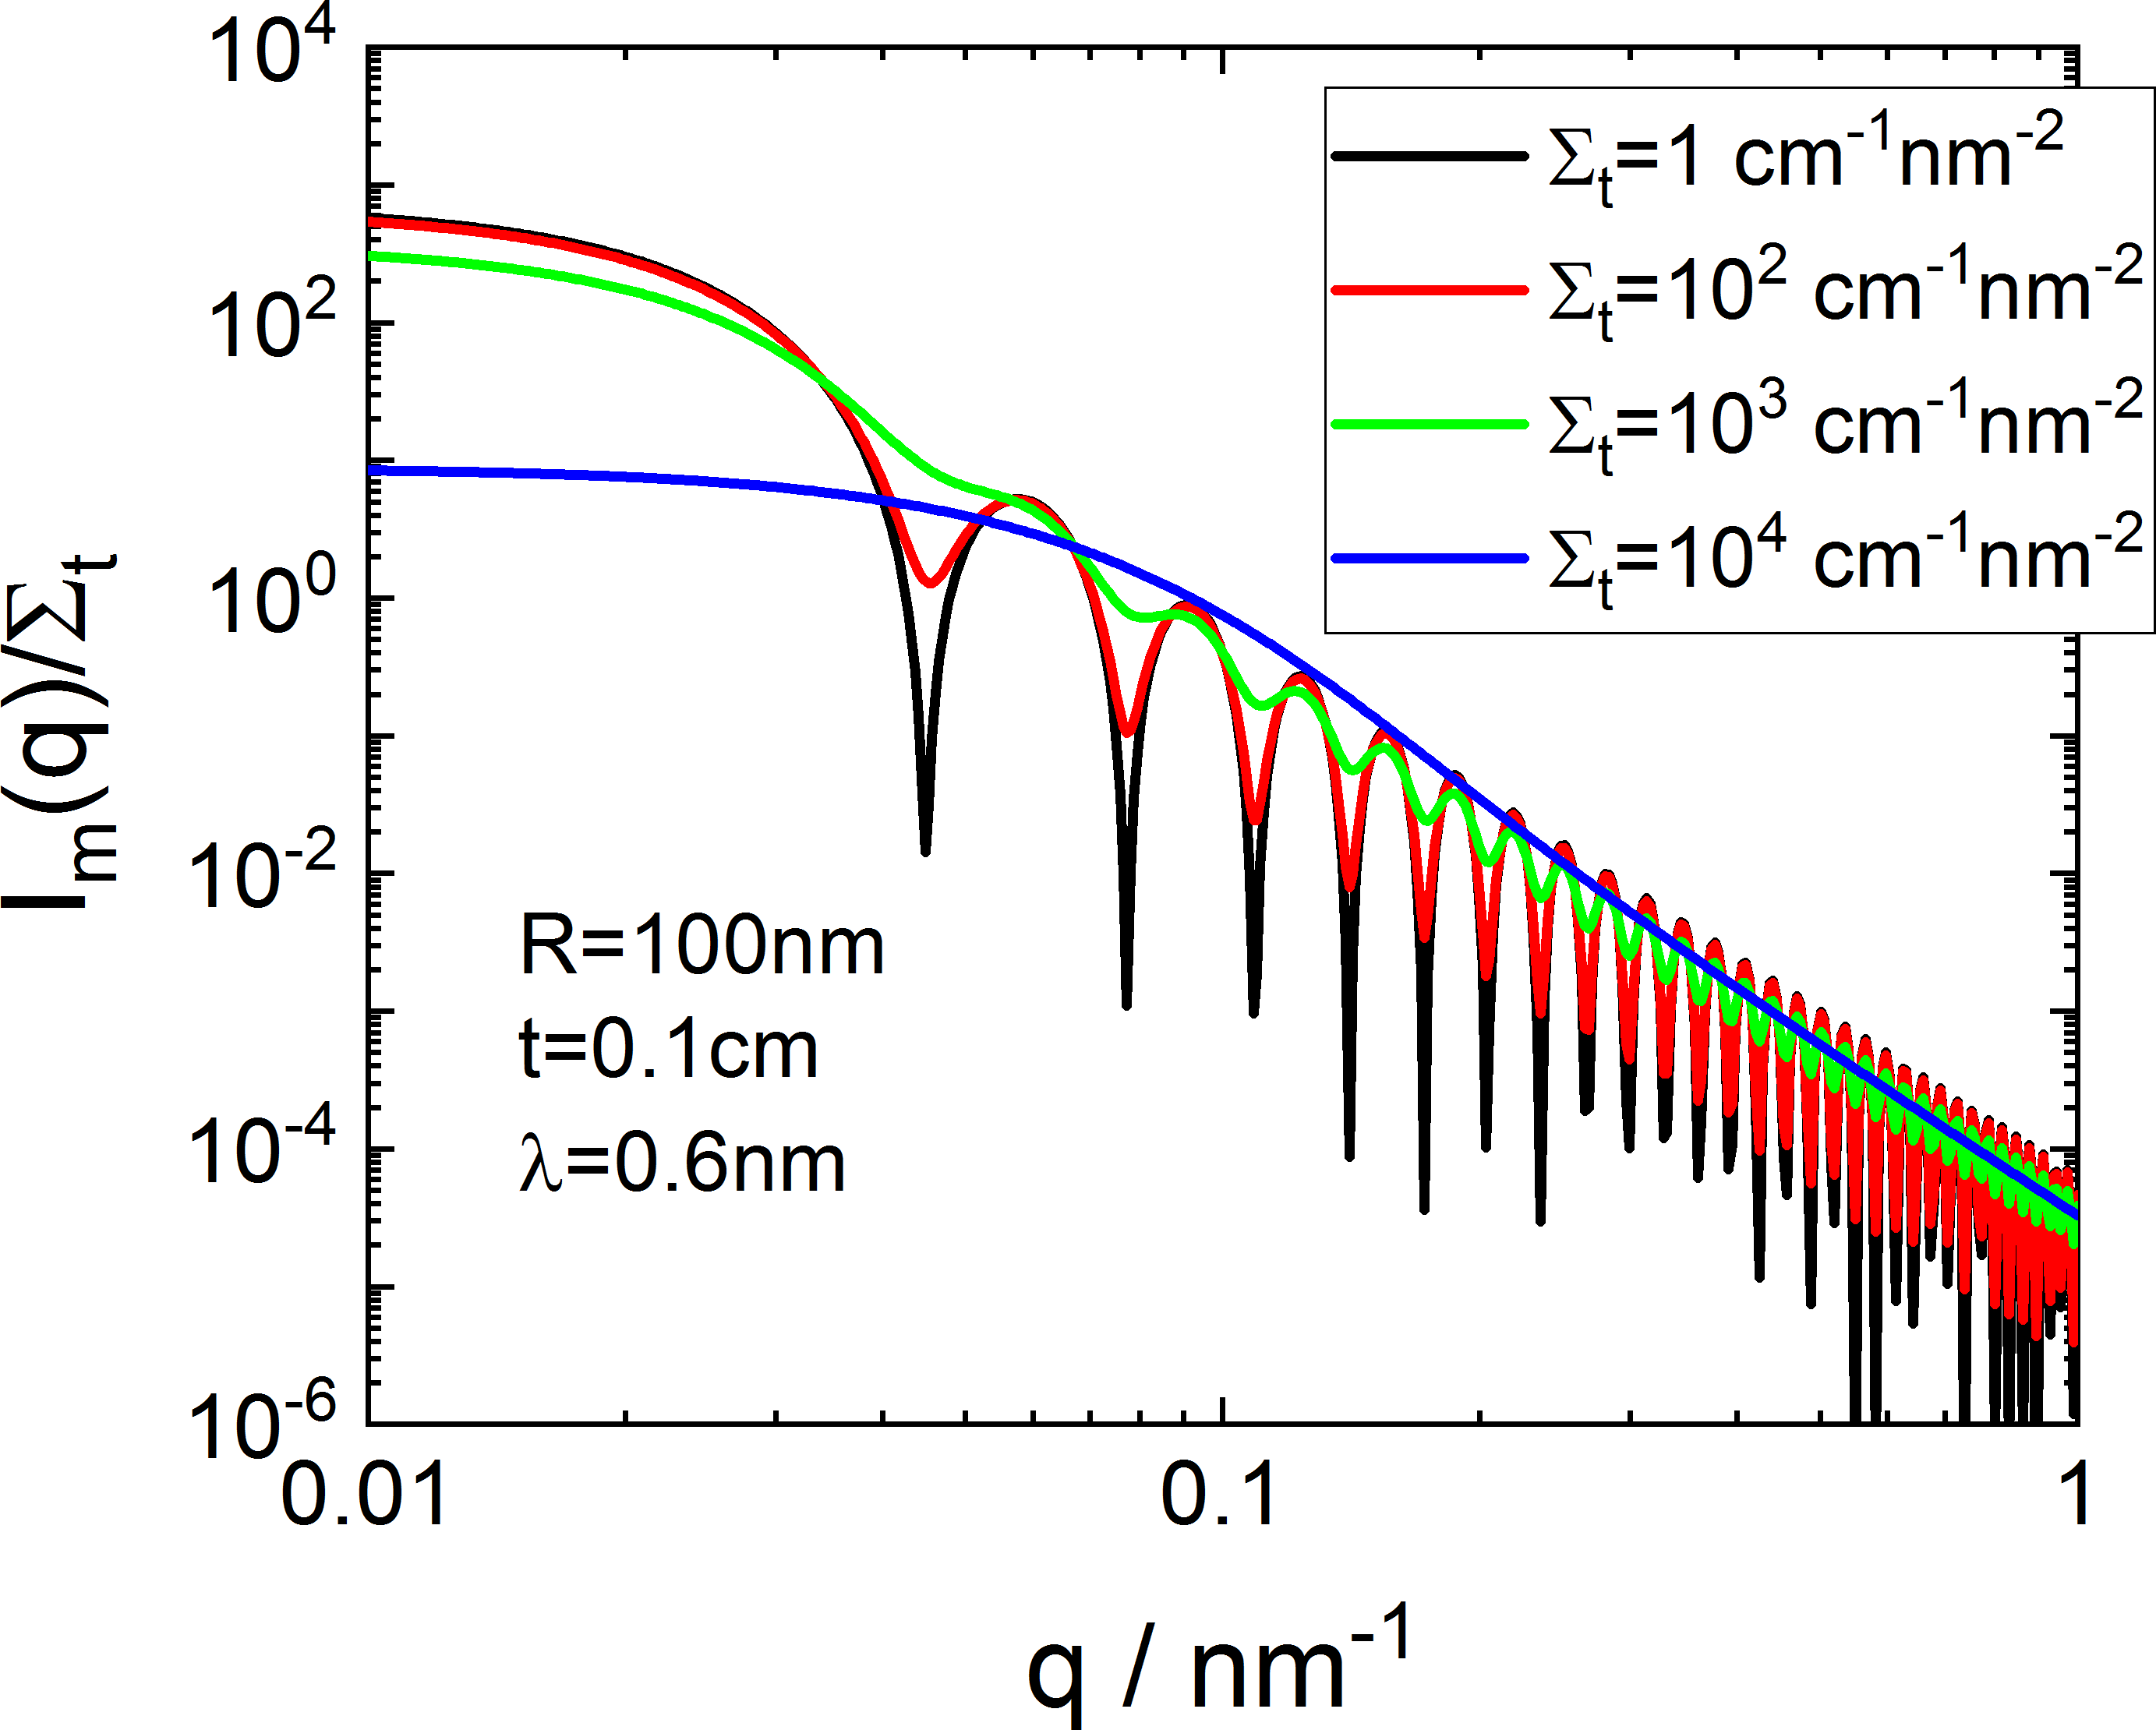
\includegraphics[width=0.7\textwidth]{../images/form_factor/MSAS/MSAS_Spheres.png}
\end{center}
\caption{Multiple scattering of monodisperse Spheres depending on their total scattering.}
\label{fig:MSAS_Spheres}
\end{figure}

\newpage
\subsection{Multiple scattering of polydisperse Spheres}

This function uses the analytical expression for projected correlation function $\tilde{G}_\mathrm{sph}(\delta)$ of monodisperse spheres as given in eq.\ \ref{eq:Gz_sph} and first integrating this function over a LogNormal distribution before combining it with eq.\ \ref{eq:MSAS_via_Gz} to calculate the scattering intensity considering multiple scattering effects.

\hspace{1pt}\\
\uline{Input Parameters for model \texttt{MSAS polydisp. Spheres}:}\\
\begin{description}
\item[\texttt{mu}] mean radius of sphere $\mu$
\item[\texttt{sigma}] LogNorm width parameter $\sigma$
\item[\texttt{dummy}] not used
\item[\texttt{Sigma\_t}] total scattering $\Sigma_t$
\item[\texttt{t}] sample thickness $t$
\item[\texttt{lambda}] wavelength of the beam $\lambda$
\end{description}

\hspace{1pt}\\
\uline{Note:}
\begin{itemize}
\item the function \texttt{MSAS polydisp. Spheres} should not be combined with a size distribution nor a structure factor.
\end{itemize}

\begin{figure}[htb]
\begin{center}
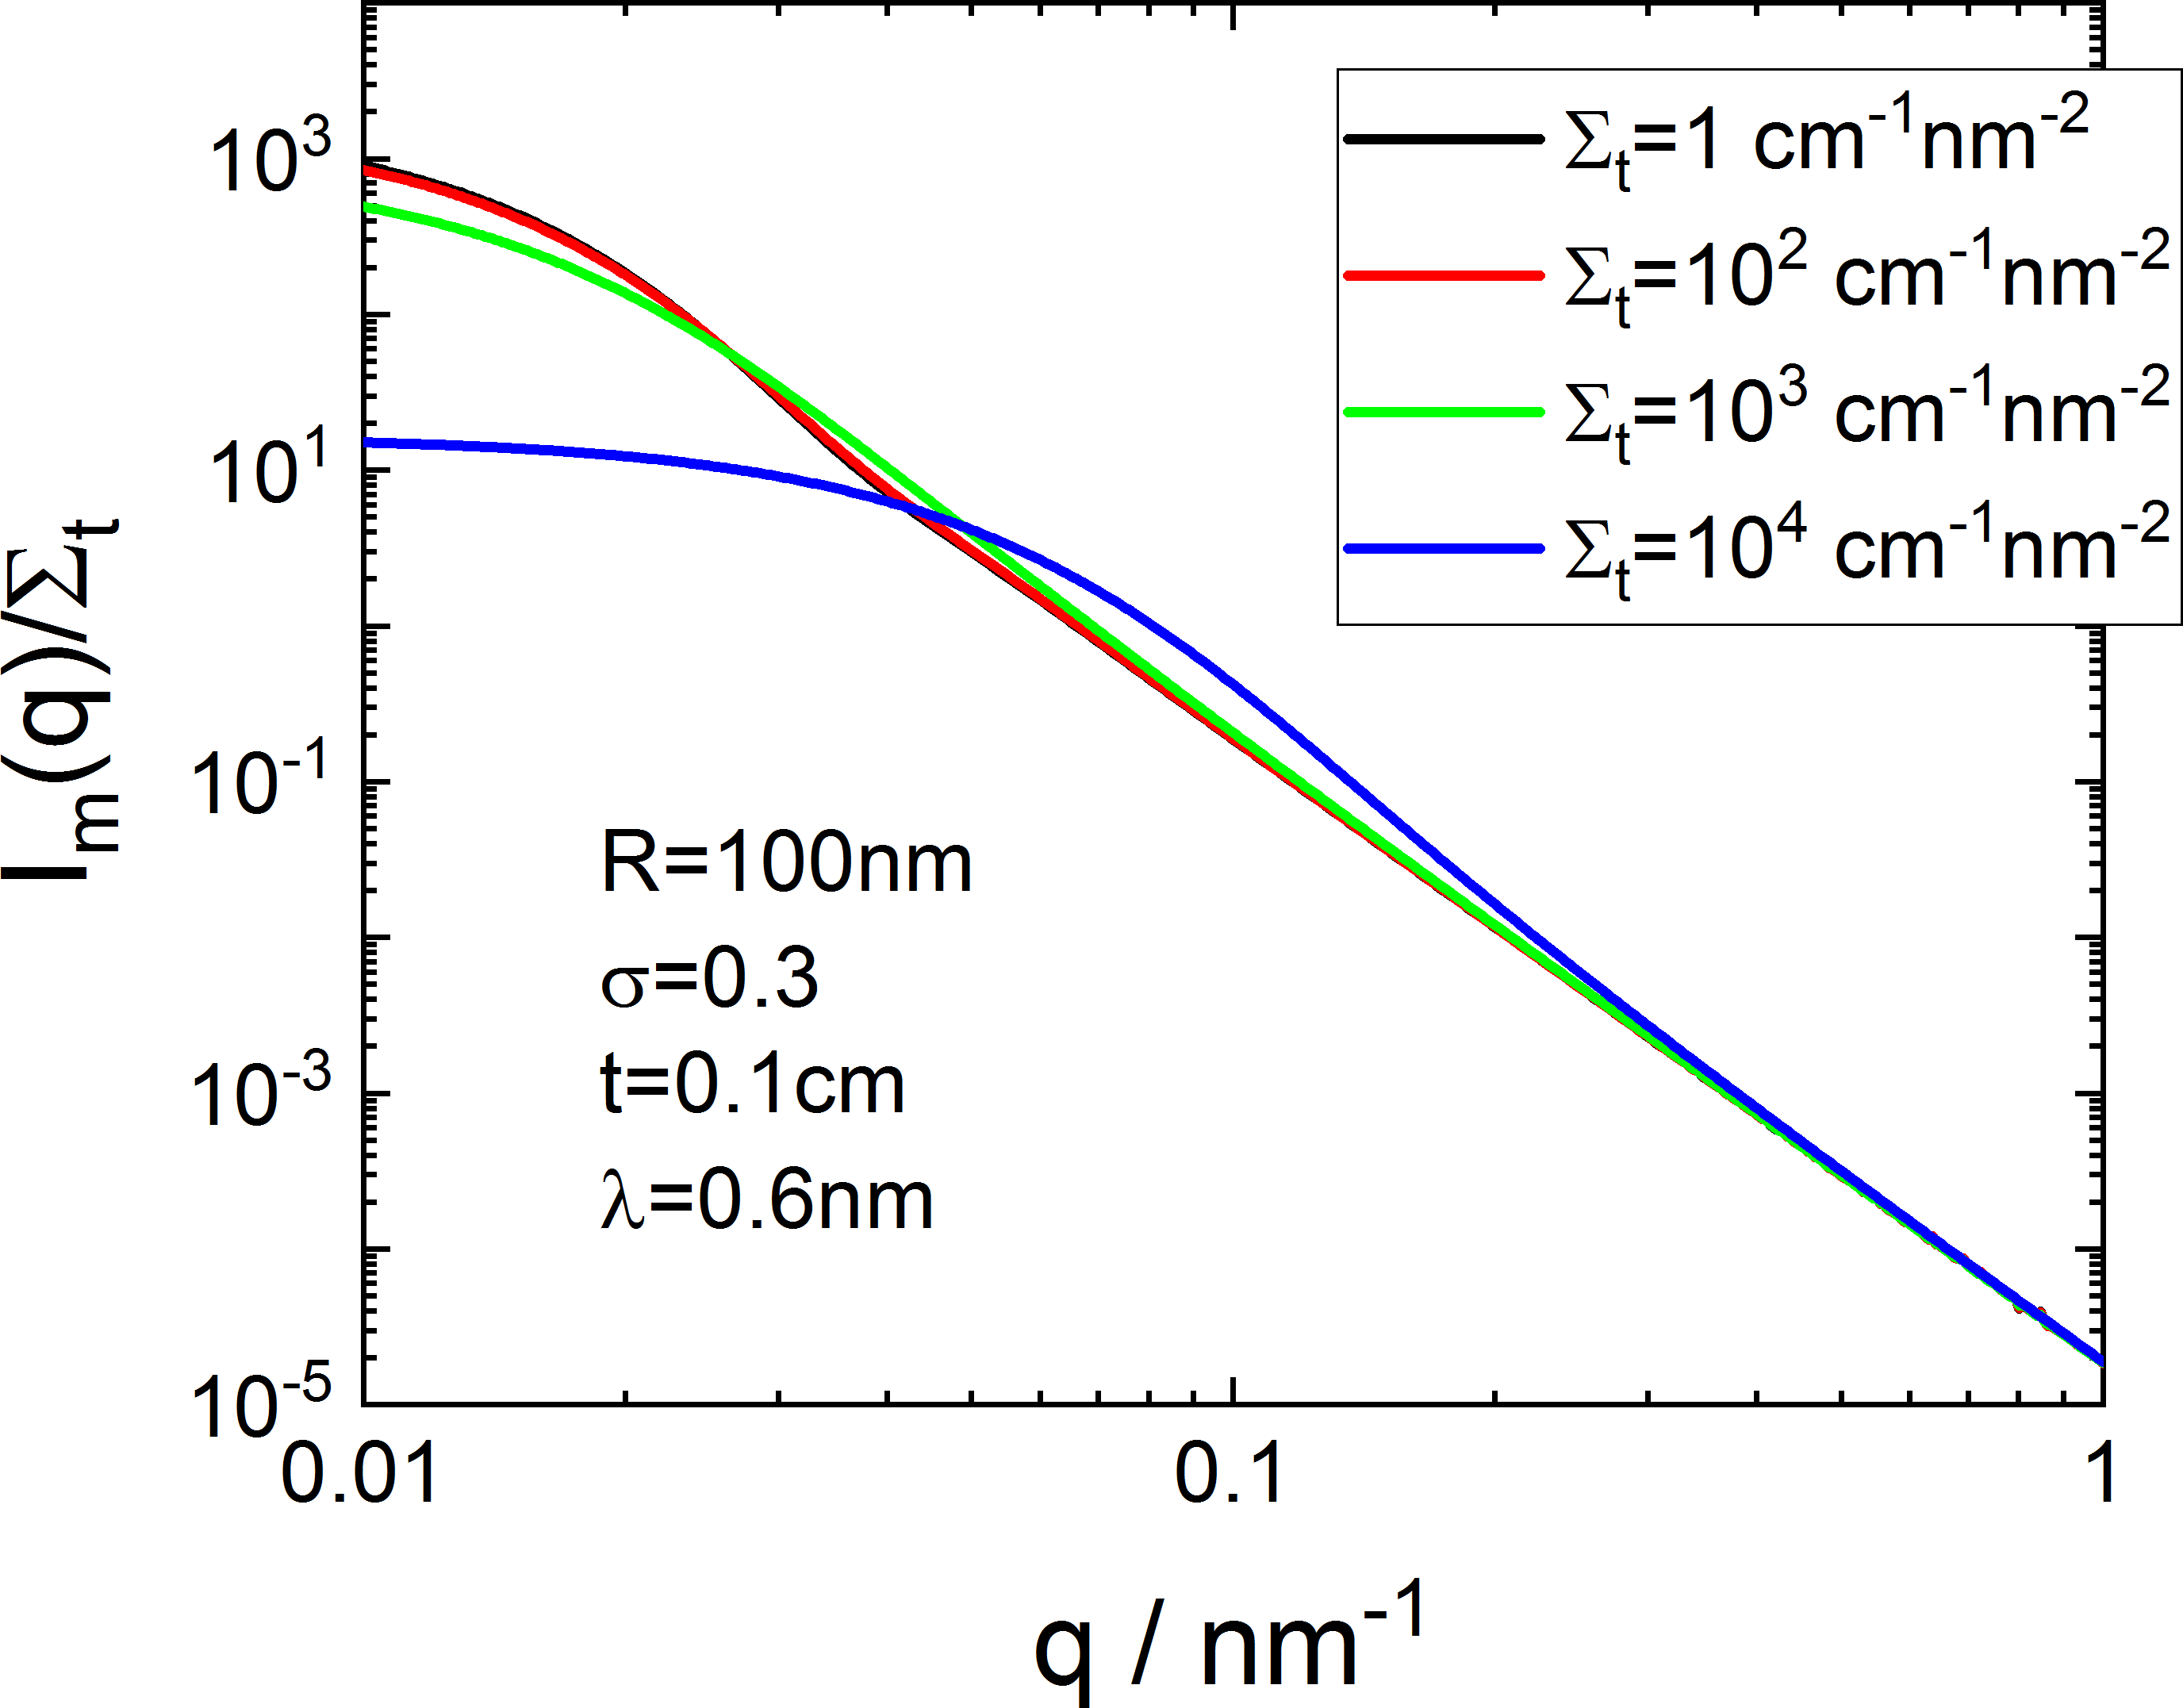
\includegraphics[width=0.7\textwidth]{../images/form_factor/MSAS/MSAS_polydispSpheres.png}
\end{center}
\caption{Multiple scattering of polydisperse Spheres following a LogNorm distribution depending on their total scattering.}
\label{fig:MSAS_polySpheres}
\end{figure}

\newpage
\subsection{Multiple scattering of Gaussian coils}

This function uses the analytical expression for projected correlation function $\tilde{G}_\mathrm{gGc}(\delta)$ of a generalised Gaussian polymer coil as given in eq.\ \ref{eq:Gz_gGc} and \ref{eq:G0_gGc} together with eq.\ \ref{eq:MSAS_via_Gz} to calculate the scattering intensity considering multiple scattering effects.

\hspace{1pt}\\
\uline{Input Parameters for model \texttt{MSAS gGc}:}\\
\begin{description}
\item[\texttt{Rg}] radius of gyration $R_g$
\item[\texttt{nu}] Flory exponent $\nu$
\item[\texttt{dummy}] not used
\item[\texttt{Sigma\_t}] total scattering $\Sigma_t$
\item[\texttt{t}] sample thickness $t$
\item[\texttt{lambda}] wavelength of the beam $\lambda$
\end{description}

\hspace{1pt}\\
\uline{Note:}
\begin{itemize}
\item the function \texttt{MSAS gGc} should not be combined with a size distribution nor a structure factor.
\item $\nu \in \left(0,\frac12\right)$
\end{itemize}

\begin{figure}[htb]
\begin{center}
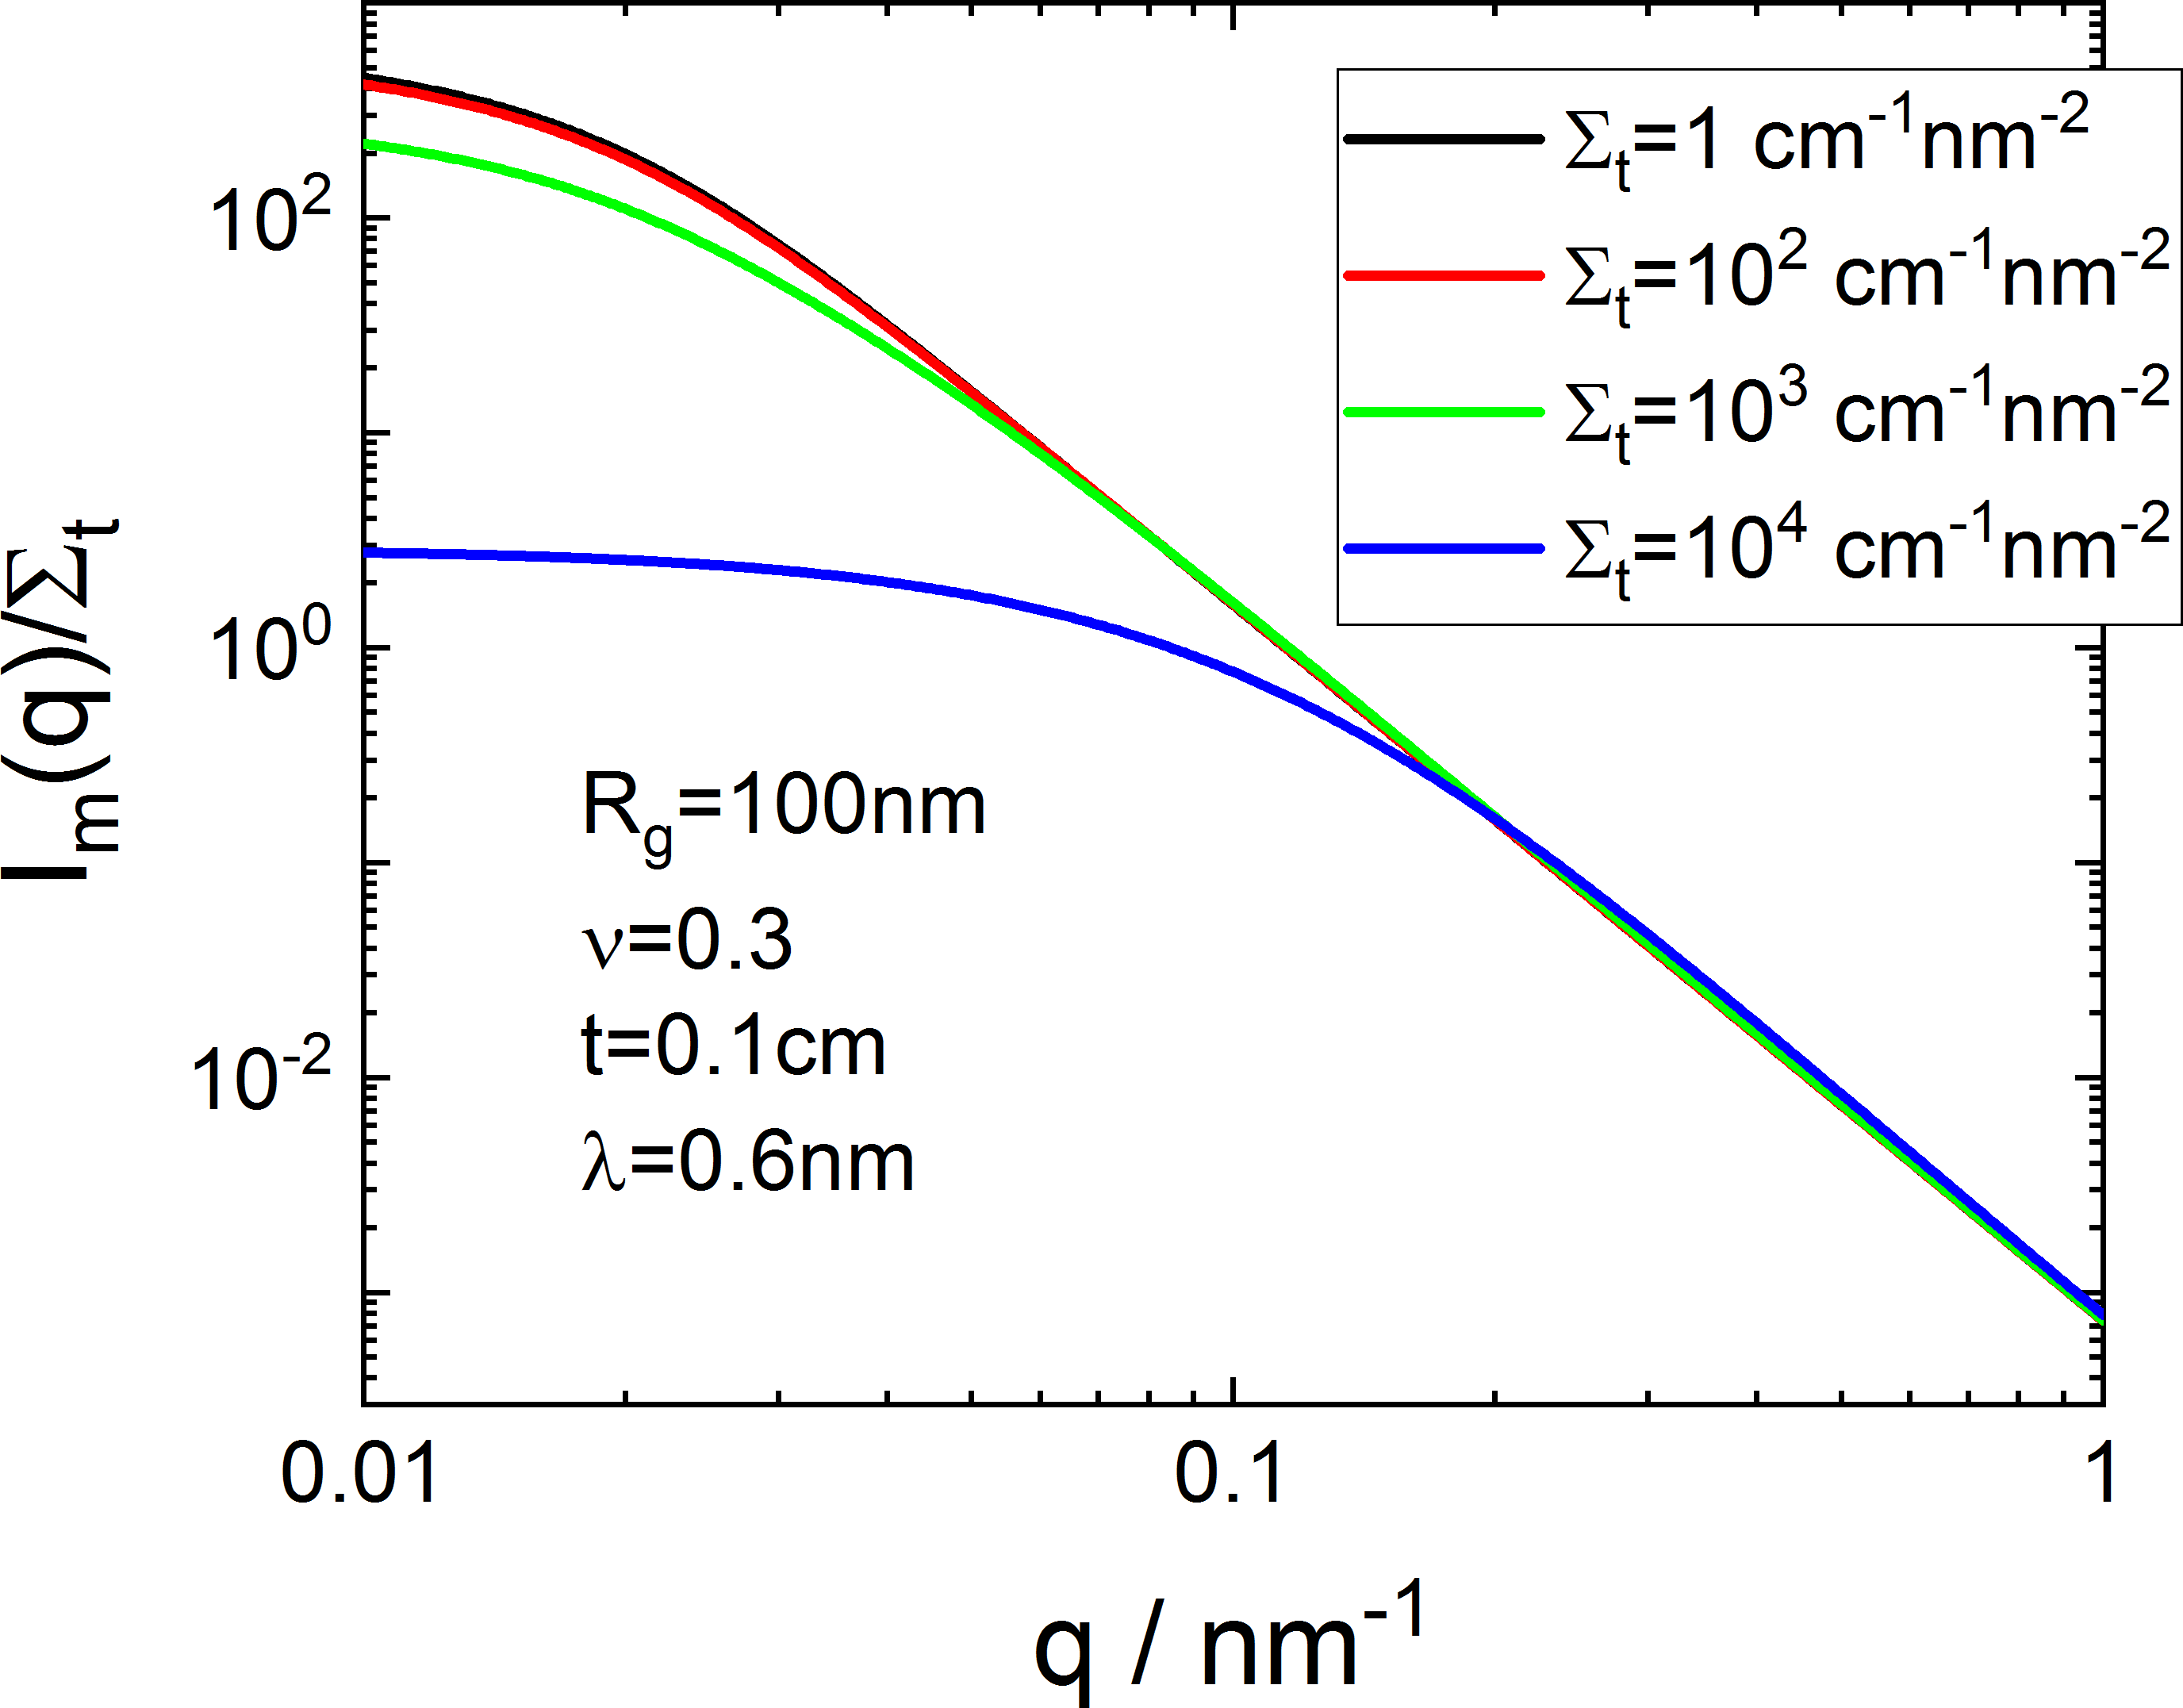
\includegraphics[width=0.7\textwidth]{../images/form_factor/MSAS/MSAS_gGc.png}
\end{center}
\caption{Multiple scattering of generalized Gaussian coil polymers depending on their total scattering.}
\label{fig:MSAS_gGc}
\end{figure}

\newpage
\subsection{Multiple scattering of a self-affine random distribution model}

This function uses the analytical expression for projected correlation function $\tilde{G}_\mathrm{gDAB}(\delta)$ of self-affine random distribution model as given in eq.\ \ref{eq:Gz_gDAB} together with eq.\ \ref{eq:MSAS_via_Gz} to calculate the scattering intensity considering multiple scattering effects.

\hspace{1pt}\\
\uline{Input Parameters for model \texttt{MSAS gDAB}:}\\
\begin{description}
\item[\texttt{xi}] correlation length $\xi$
\item[\texttt{H}] Hurst exponent $H$
\item[\texttt{dummy}] not used
\item[\texttt{Sigma\_t}] total scattering $\Sigma_t$
\item[\texttt{t}] sample thickness $t$
\item[\texttt{lambda}] wavelength of the beam $\lambda$
\end{description}

\hspace{1pt}\\
\uline{Note:}
\begin{itemize}
\item the function \texttt{MSAS gDAB} should not be combined with a size distribution nor a structure factor.
\item $H$ needs to be positive and non-zero: $H > 0$
\end{itemize}

\begin{figure}[htb]
\begin{center}
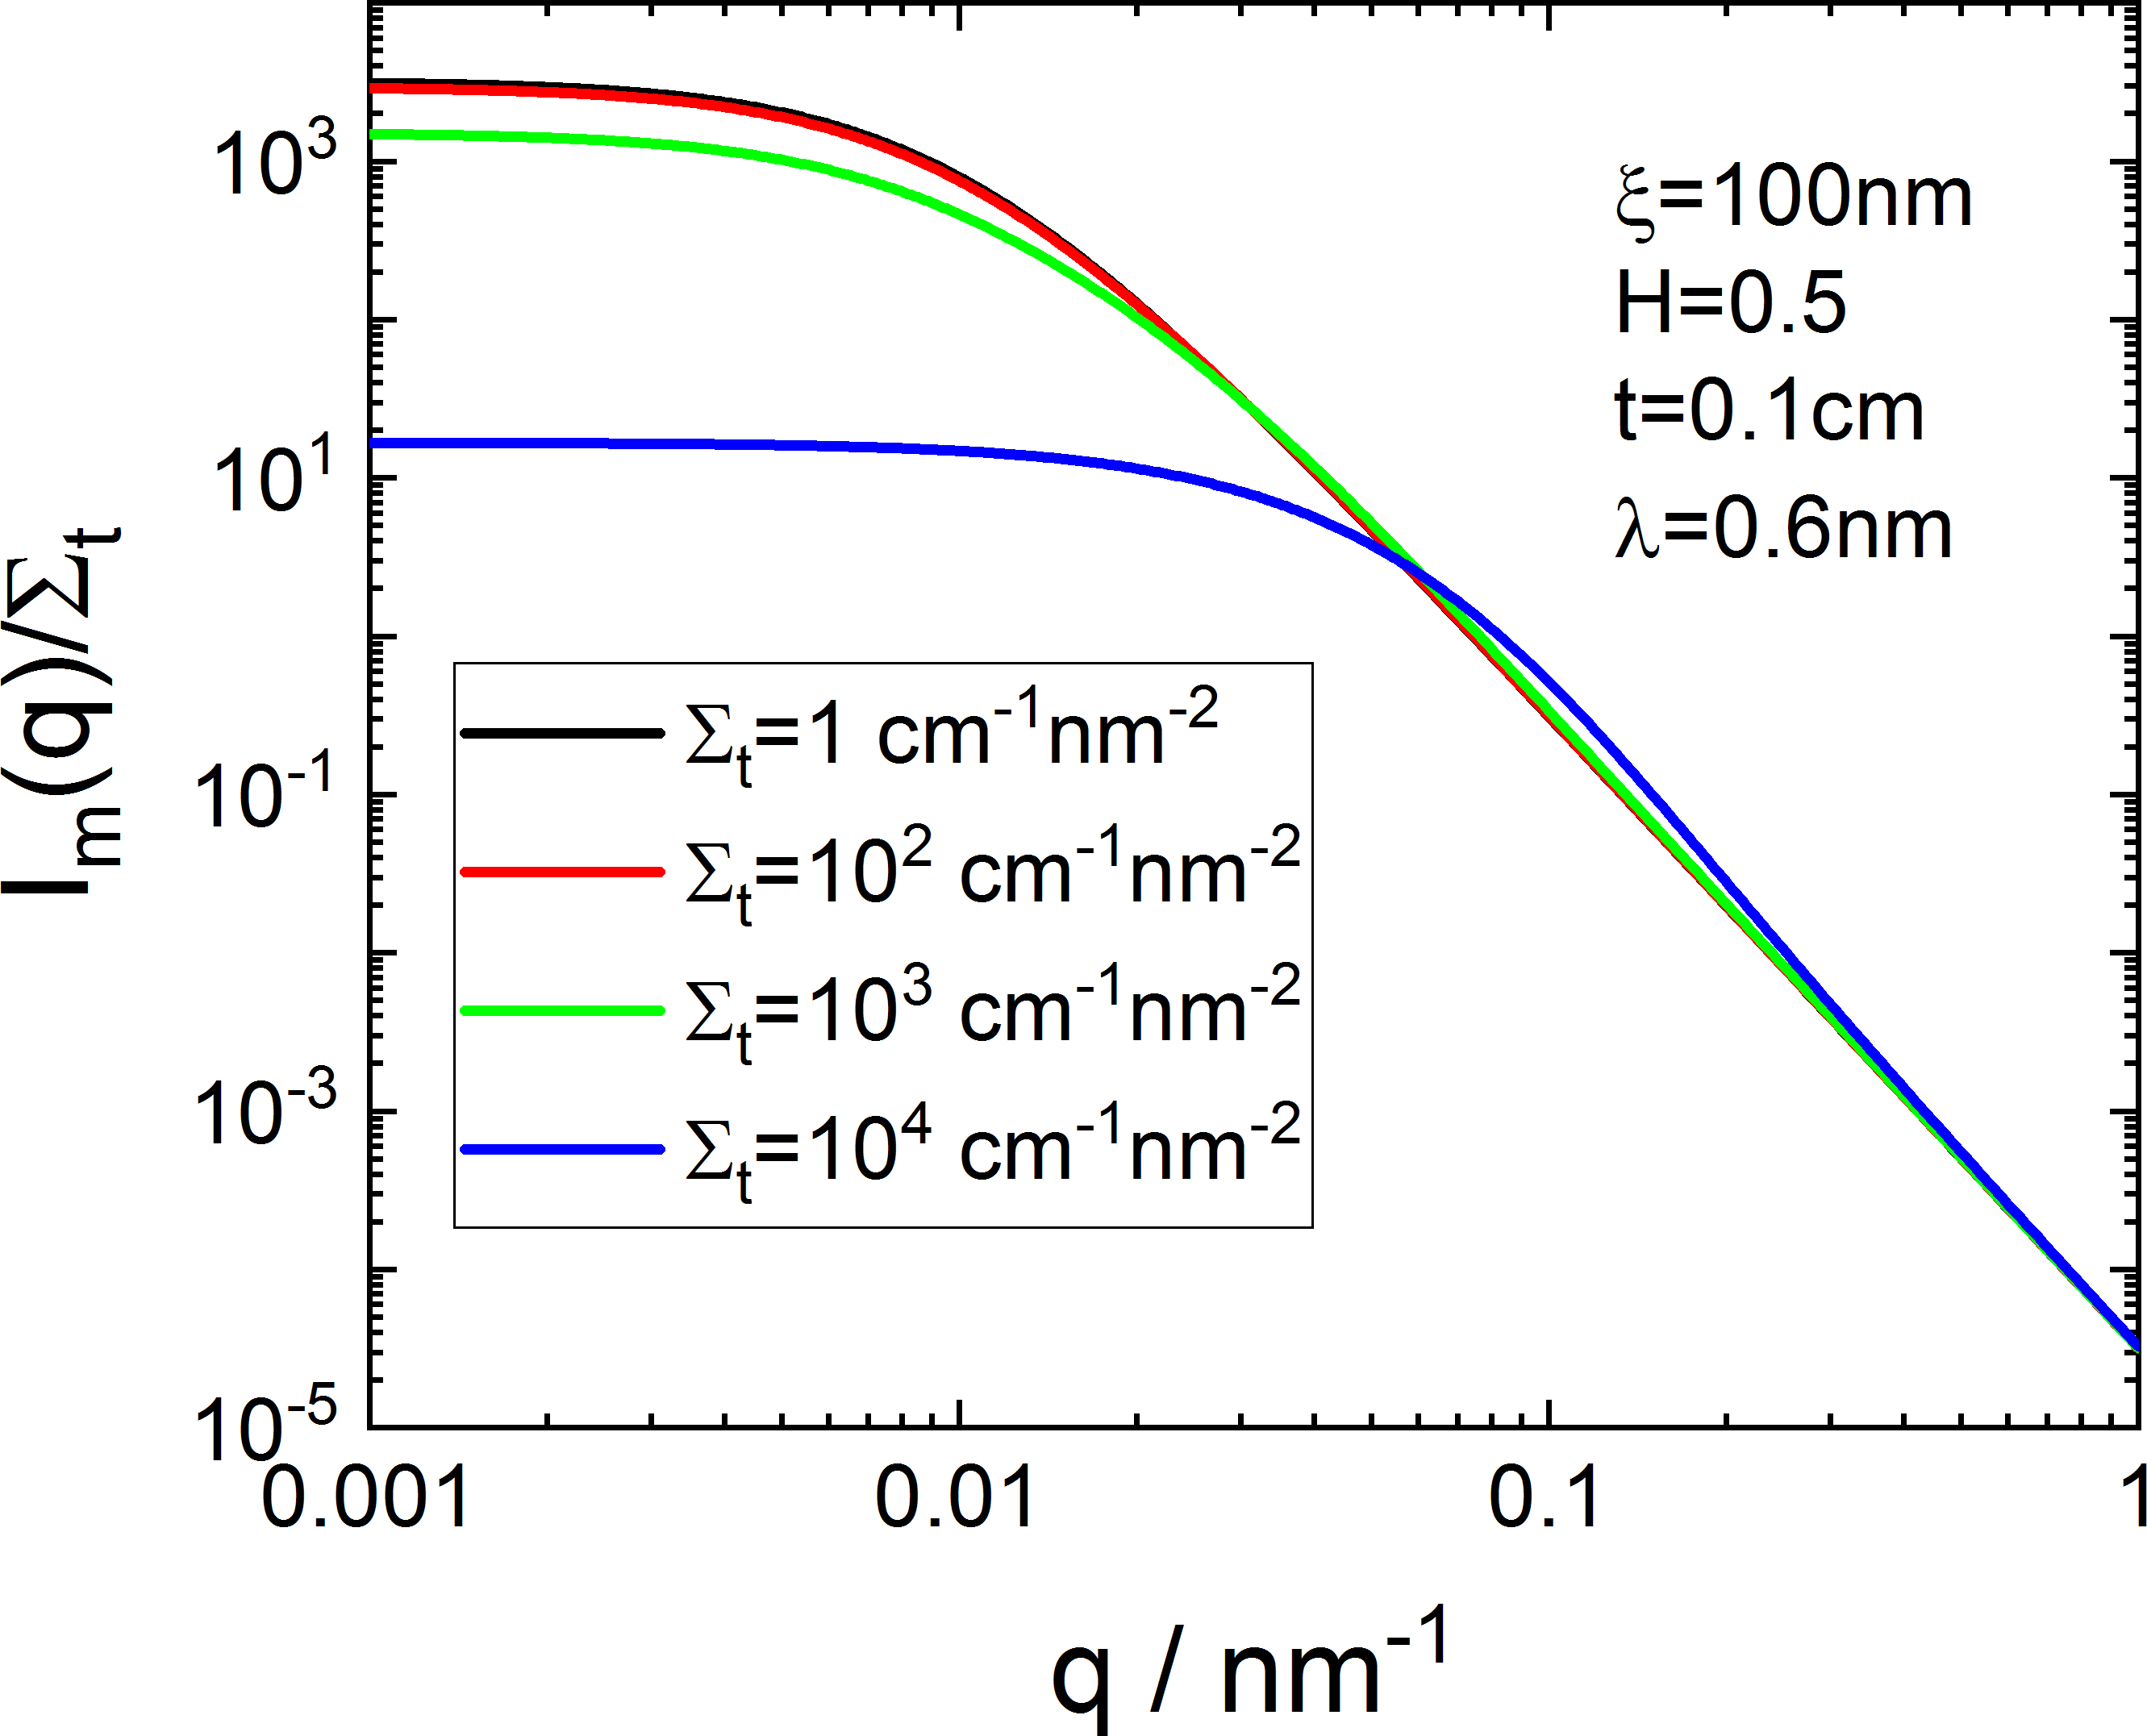
\includegraphics[width=0.7\textwidth]{../images/form_factor/MSAS/MSAS_gDAB.png}
\end{center}
\caption{Multiple scattering of self-affine random distributions (gDAB) model depending on their total scattering.}
\label{fig:MSAS_gDAB}
\end{figure} 